\documentclass[
  a4paper,
  oneside,
  BCOR = 10mm,
  DIV = 12,
  12pt,
  headings = normal,
]{scrartcl}

%%% Length calculations
\usepackage{calc}
%%%

%%% Support for color
\usepackage{xcolor}
\definecolor{lightblue}{HTML}{03A9F4}
\definecolor{red}{HTML}{F44336}
%%%

%%% Including graphics
\usepackage{graphicx}
%%%

%%% Font selection
\usepackage{fontspec}

\setromanfont{STIX Two Text}[
  SmallCapsFeatures = {LetterSpace = 8},
]

\setsansfont{IBM Plex Sans}[
  Scale = MatchUppercase,
]

\setmonofont{IBM Plex Mono}[
  Scale = MatchUppercase,
]
%%%

%%% Math typesetting
\usepackage{amsmath}

\usepackage{unicode-math}
\setmathfont{STIX Two Math}

\usepackage{IEEEtrantools}
%%%

%%% List settings
\usepackage{enumitem}
\setlist[enumerate]{
  label*      = {\arabic*.},
  left        = \parindent,
  topsep      = 0\baselineskip,
  parsep      = 0\baselineskip,
  noitemsep, % override itemsep
}
% List settings for levels 2–4
\setlist[enumerate, 2, 3, 4]{
  label*      = {\arabic*.},
  left        = 0em,
  topsep      = 0\baselineskip,
  parsep      = 0\baselineskip,
  noitemsep, % override itemsep
}

\setlist[itemize]{
  label*      = {—},
  left        = \parindent,
  topsep      = 0\baselineskip,
  parsep      = 0\baselineskip,
  itemsep     = 1\baselineskip,
  noitemsep, % override itemsep
}

\setlist[description]{
  font        = {\rmfamily\upshape\bfseries},
  topsep      = 1\baselineskip,
  parsep      = 0\baselineskip,
  itemsep     = 0\baselineskip,
}

%%%

%%% Structural elements typesetting
\setkomafont{pagenumber}{\rmfamily\upshape}
\setkomafont{disposition}{\rmfamily\bfseries}

% Sectioning
\RedeclareSectionCommand[
  beforeskip = -1\baselineskip,
  afterskip  = 1\baselineskip,
  font       = {\normalsize\bfseries\scshape},
]{section}

\RedeclareSectionCommand[
  beforeskip = -1\baselineskip,
  afterskip  = 1\baselineskip,
  font       = {\normalsize\bfseries\itshape},
]{subsection}

\RedeclareSectionCommand[
  beforeskip = -1\baselineskip,
  afterskip  = 1\baselineskip,
  font       = {\normalsize\bfseries},
]{subsubsection}

\RedeclareSectionCommand[
  beforeskip = -1\baselineskip,
  afterskip  = -0.5em,
  font       = {\normalsize\mdseries\scshape\addfontfeatures{Letters = {UppercaseSmallCaps}}},
]{paragraph}
%%%

%%% Typographic enhancements
\usepackage{microtype}
%%%

%%% Language-specific settings
\usepackage{polyglossia}
\setmainlanguage{ukrainian}
\setotherlanguages{english}
%%%

%%% Captions
\usepackage{caption}
\usepackage{subcaption}

%\DeclareCaptionLabelFormat{closing}{#2)}
%\captionsetup[subtable]{labelformat = closing}

%\captionsetup[subfigure]{labelformat = closing}

\captionsetup[table]{
  aboveskip = 0\baselineskip,
  belowskip = 0\baselineskip,
}

\captionsetup[figure]{
  aboveskip = 1\baselineskip,
  belowskip = 0\baselineskip,
}

\captionsetup[subfigure]{
  labelformat = simple,
  labelformat = brace,
  justification = RaggedRight,
  singlelinecheck = false,
}
%%%

%%% Hyphenated ragged typesetting
\usepackage{ragged2e}
%%%

%%% Table typesetting
\usepackage{booktabs}
\usepackage{longtable}

\usepackage{multirow}

\usepackage{array}
\newcolumntype{v}[1]{>{\RaggedRight\arraybackslash\hspace{0pt}}p{#1}}
\newcolumntype{b}[1]{>{\Centering\arraybackslash\hspace{0pt}}p{#1}}
\newcolumntype{n}[1]{>{\RaggedLeft\arraybackslash\hspace{0pt}}p{#1}}
%%%

%%% Drawing
\usepackage{tikz}
\usepackage{tikzscale}
\usetikzlibrary{arrows.meta} % Stealth arrow tips
\usetikzlibrary{backgrounds} % Stealth arrow tips
\usetikzlibrary{datavisualization.formats.functions}
\usetikzlibrary{datavisualization}
\usetikzlibrary{fit}
\usetikzlibrary{graphdrawing}
\usegdlibrary{trees}
\usetikzlibrary{graphs}
\usetikzlibrary{intersections}
\usetikzlibrary{patterns}
\usetikzlibrary{positioning}
\usetikzlibrary{shapes.geometric}
\usetikzlibrary{quotes}

\usepackage{pgfplots}
\usepgfplotslibrary{fillbetween}
%%%

%%% SI units typesetting
\usepackage{siunitx}
\sisetup{
  output-decimal-marker = {,},
  exponent-product      = {\cdot},
  inter-unit-product    = \ensuremath{{} \cdot {}},
  per-mode              = symbol,
}
%%%

% Code Highlighting
\usepackage{minted}
\setmintedinline{
  style = bw,
  breaklines,
}

\newminted[bashterm]{text}{%
  autogobble,%
  breaklines,%
  style=bw,%
}

\newminted[codegeneric]{text}{%
  autogobble,%
  style=bw,%
  breaklines,%
  fontsize=\small,%
}

\newmintinline{bash}{%
}

\newmintinline[minttext]{text}{%
  breaklines,%
  breakanywhere,%
}

%%% Framing code listings
\usepackage{tcolorbox}
\tcbuselibrary{breakable}
\tcbuselibrary{minted}
\tcbuselibrary{skins}

% Text file listing
\newtcblisting[
  auto counter,
  list inside,
  number within = section,
]{listingplaintext}[3][]{%
  minted language = text,
  minted style    = bw,
  minted options  = {
    autogobble,
    linenos,
    tabsize = 4,
    breaklines,
    breakanywhere,
    fontsize = \footnotesize,
  },
  empty,
  sharp corners,
  coltitle = black,
  borderline horizontal = {1pt}{0pt}{black},
  titlerule = {0.5pt},
  titlerule style = {
    black,
  },
  toptitle = 0.3em,
  bottomtitle = 0.3em,
  before skip      = \intextsep,
  after  skip      = \intextsep,
  title            = {Лістинг \thetcbcounter: #2},
  list entry       = {\protect\numberline{\thetcbcounter}#2},
  left = 0em,
  right = 0em,
  %
  listing only,
  breakable,
  %
  label = {#3},%
}

\newtcbinputlisting[
  use counter from = listingplaintext,
  list inside,
  number within = section
]{\inputplaintext}[4][]{%
  minted language = text,
  minted style    = bw,
  minted options  = {
    autogobble,
    linenos,
    tabsize = 4,
    breaklines,
    breakanywhere,
    fontsize = \footnotesize,
  },
  empty,
  sharp corners,
  coltitle = black,
  borderline horizontal = {1pt}{0pt}{black},
  titlerule = {0.5pt},
  titlerule style = {
    black,
  },
  toptitle = 0.3em,
  bottomtitle = 0.3em,
  before skip      = \intextsep,
  after  skip      = \intextsep,
  title            = {Лістинг \thetcbcounter: #3},
  list entry       = {\protect\numberline{\thetcbcounter}#3},
  left = 0em,
  right = 0em,
  %
  listing file={#2},
  listing only,
  breakable,
  %
  label = {#4}
}

\newtcblisting[
  use counter from = listingplaintext,
  list inside,
  number within = section,
]{listingpython}[3][]{%
  minted language = python,
  minted style    = bw,
  minted options  = {
    autogobble,
    linenos,
    tabsize = 4,
    breaklines,
    breakanywhere,
    fontsize = \footnotesize,
  },
  empty,
  sharp corners,
  coltitle = black,
  borderline horizontal = {1pt}{0pt}{black},
  titlerule = {0.5pt},
  titlerule style = {
    black,
  },
  toptitle = 0.3em,
  bottomtitle = 0.3em,
  before skip      = \intextsep,
  after  skip      = \intextsep,
  title            = {Лістинг \thetcbcounter: #2},
  list entry       = {\protect\numberline{\thetcbcounter}#2},
  left = 0em,
  right = 0em,
  %
  listing only,
  breakable,
  %
  label = {#3},
  %
  #1%
}

\newtcbinputlisting[
  use counter from = listingplaintext,
  list inside,
  number within = section
]{\inputpython}[4][]{%
  minted language = python,
  minted style    = bw,
  minted options  = {
    autogobble,
    linenos,
    tabsize = 4,
    breaklines,
    breakanywhere,
    fontsize = \footnotesize,
  },
  empty,
  sharp corners,
  coltitle = black,
  borderline horizontal = {1pt}{0pt}{black},
  titlerule = {0.5pt},
  titlerule style = {
    black,
  },
  toptitle = 0.3em,
  bottomtitle = 0.3em,
  before skip      = \intextsep,
  after  skip      = \intextsep,
  title            = {Лістинг \thetcbcounter: #3},
  list entry       = {\protect\numberline{\thetcbcounter}#3},
  left = 0em,
  right = 0em,
  %
  listing file={#2},
  listing only,
  breakable,
  %
  label = {#4}
}

\newtcbinputlisting[
  use counter from = listingplaintext,
  list inside,
  number within = section
]{\inputada}[4][]{%
  minted language = ada,
  minted style    = bw,
  minted options  = {
    autogobble,
    linenos,
    tabsize = 4,
    breaklines,
    breakanywhere,
    fontsize = \footnotesize,
  },
  empty,
  sharp corners,
  coltitle = black,
  borderline horizontal = {1pt}{0pt}{black},
  titlerule = {0.5pt},
  titlerule style = {
    black,
  },
  toptitle = 0.3em,
  bottomtitle = 0.3em,
  before skip      = \intextsep,
  after  skip      = \intextsep,
  title            = {Лістинг \thetcbcounter: #3},
  list entry       = {\protect\numberline{\thetcbcounter}#3},
  left = 0em,
  right = 0em,
  %
  listing file={#2},
  listing only,
  breakable,
  %
  label = {#4}
}

% Linux command-line listing
\newtcblisting{linuxterm}%
{%
  % Syntax highlighing options
  listing only,%
  minted language = bash,%
  minted options={%
    autogobble,%
    linenos%
  },%
  % Presentation options
  empty,%
  %% Margins
  sharp corners,%
  toptitle = 0.0em,%
  bottomtitle = 0.0em,%
  left = 0em,%
  right = 0em,%
  before skip = \intextsep,%
  after skip = \intextsep,%
}

\newtcblisting{linuxtermout}%
{%
  % Syntax highlighing options
  listing only,%
  minted language = text,%
  minted options={%
    autogobble,%
    linenos%
  },%
  % Presentation options
  empty,%
  %% Margins
  sharp corners,%
  toptitle = 0.0em,%
  bottomtitle = 0.0em,%
  left = 0em,%
  right = 0em,%
  before skip = \intextsep,%
  after skip = \intextsep,%
}

% Dockerfile listings
\newtcblisting[
  use counter from = listingplaintext,
  list inside,
  number within = section,
]{listingdocker}[3][]{%
  minted language = dockerfile,
  minted style    = bw,
  minted options  = {
    autogobble,%
    linenos,
    tabsize = 4,
    breaklines,
    breakanywhere,
    fontsize = \footnotesize,
  },
  empty,
  sharp corners,
  coltitle = black,
  borderline horizontal = {1pt}{0pt}{black},
  titlerule = {0.5pt},
  titlerule style = {
    black,
  },
  toptitle = 0.3em,
  bottomtitle = 0.3em,
  before skip      = \intextsep,
  after  skip      = \intextsep,
  title            = {Лістинг \thetcbcounter: #2},
  list entry       = {\protect\numberline{\thetcbcounter}#2},
  left = 0em,
  right = 0em,
  %
  listing only,
  breakable,
  %
  label = {#3},%
}

% Docker Compose listings
\newtcblisting[
  use counter from = listingplaintext,
  list inside,
  number within = section,
]{listingdockercompose}[3][]{%
  minted language = yaml,
  minted style    = bw,
  minted options  = {
    autogobble,%
    linenos,
    tabsize = 4,
    breaklines,
    breakanywhere,
    fontsize = \footnotesize,
  },
  empty,
  sharp corners,
  coltitle = black,
  borderline horizontal = {1pt}{0pt}{black},
  titlerule = {0.5pt},
  titlerule style = {
    black,
  },
  toptitle = 0.3em,
  bottomtitle = 0.3em,
  before skip      = \intextsep,
  after  skip      = \intextsep,
  title            = {Лістинг \thetcbcounter: #2},
  list entry       = {\protect\numberline{\thetcbcounter}#2},
  left = 0em,
  right = 0em,
  %
  listing only,
  breakable,
  %
  label = {#3},%
}


% Customize minted line numbers
\renewcommand{\theFancyVerbLine}{\ttfamily\scriptsize\arabic{FancyVerbLine}}

%%%

%%% Typeset menus and keys
\usepackage{menukeys}[
  os=win,
]
%%%

%%% Links and hyperreferences
\usepackage{hyperref}
\hypersetup{
  bookmarksnumbered = true,
  colorlinks      = false,
  linkbordercolor = red,
  urlbordercolor  = lightblue,
  pdfborderstyle  = {/S/U/W 1.5},
}
%%%

%%% Length adjustment

% Set baselineskip, default is 14.5 pt
\linespread{1.068966} % ~15.5 pt
\setlength{\emergencystretch}{1em}
\setlength{\parindent}{1.5em}
\newlength{\gridunitwidth}
\setlength{\gridunitwidth}{\textwidth / 12}
%%%

%%% Custom commands
\newcommand{\allcaps}[1]{%
  {%
    \addfontfeatures{%
      Letters = UppercaseSmallCaps,
      LetterSpace = 8,%
    }%
    #1%
  }%
}
\newcommand{\filename}[1]{\texttt{#1}}
\newcommand{\progname}[1]{\texttt{#1}}
\newcommand{\commandname}[1]{\texttt{#1}}
\newcommand{\modulename}[1]{\texttt{#1}}
\newcommand{\transeng}[1]{{англ.}~\textit{\textenglish{#1}}}
%%%

%%% Custom math commands
\newcommand{\longvar}[1]{\mathit{#1}}
\newcommand{\vect}[1]{\mathbfit{#1}}
\newcommand{\matr}[1]{\mathbfit{#1}}

\newcommand{\logequiv}{\mathrel{\Longleftrightarrow}} % Logically equivalent

\DeclareMathOperator*{\minimize}{min} % minimize for linear programs
%%%

%%% Custom drawing commands
\makeatletter
\newcommand{\Distance}[3]{% % from https://tex.stackexchange.com/q/56353/121799
\tikz@scan@one@point\pgfutil@firstofone($#1-#2$)\relax  
\pgfmathsetmacro{#3}{veclen(\the\pgf@x,\the\pgf@y)}
}% Explanation: the calc library allows us, among other things, to add and
% subtract points, so ($#1-#2$) is simply the difference between the points
% #1 and #2. The combination \tikz@scan@one@point\pgfutil@firstofone extracts
% the coordinates of the new point and stores them in \pgf@x and \pgf@y.
% They get fed in veclen, and \pgfmathsetmacro stores the result in #3.
% EDIT: included fudge factor, see https://tex.stackexchange.com/a/22702/121799
\makeatother
%%%

\begin{document}

\begin{titlepage}
    \begin{center}
      Міністерство освіти і~науки України\\
      Національний авіаційний університет\\
      Факультет кібербезпеки, комп'ютерної та~програмної інженерії\\
      Кафедра комп'ютеризованих систем управління

      \vspace{\fill}
        Лабораторна робота №~1.4\\
        з~дисципліни «Паралельні і~розподілені обчислення»\\
        на~тему «Монітори»

      \vspace{\fill}

      \begin{flushright}
        Виконав:\\
        студент \allcaps{ФККПІ}\\
        групи \allcaps{СП}-425\\
        Клокун В.\,Д.\\
        Перевірив:\\
        Корочкін О.\,В.
      \end{flushright}

      Київ 2019
    \end{center}
  \end{titlepage}

  \section{Завдання роботи}
    Розробити програму для~заданої паралельної комп'ютерної системи зі~спільною пам'яттю~(рис.~\ref{fig:task-sys}).

    \begin{figure}[!htbp]
      \centering
      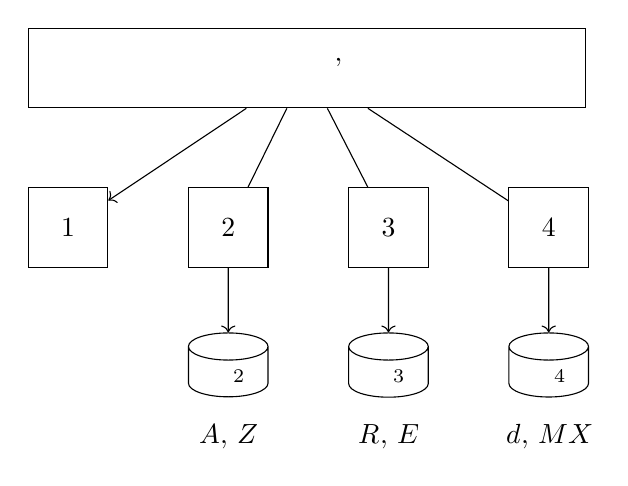
\begin{tikzpicture}[
        iod/.style = {
          draw,
          cylinder,
          shape border rotate = 90,
          minimum width = \gridunitwidth,
          aspect = 0.5,
        },
        memd/.style = {
          draw,
          rectangle,
          minimum height = 1\gridunitwidth,
          minimum width = 7\gridunitwidth,
        },
        thread/.style = {
          draw,
          rectangle,
          minimum width = \gridunitwidth,
          minimum height = \gridunitwidth,
        }
      ]
        \node (mem) at (0,0) [
          memd,
        ] {Спільна пам'ять};

        \node (t1) [
          thread,
          below = of mem.south west,
          anchor = north west,
        ] {1};

        % \node (iod1) [
        %   iod,
        %   below = of t1.south west,
        %   anchor = before top,
        % ] {$\text{ПВВ}_{1}$};

        % \node (vars1) [
        %   below = 0.5 \baselineskip of iod1,
        % ] {$MA, MB$};

        \node (t2) [
          thread,
          right = 1\gridunitwidth of t1.north east,
          anchor = north west,
        ] {2};

        \node (iod2) [
          iod,
          below = of t2.south west,
          anchor = before top,
        ] {$\text{ПВВ}_{2}$};

        \node (vars2) [
          below = 0.5 \baselineskip of iod2,
        ] {$A, \, Z$};

        \node (t3) [
          thread,
          right = 1\gridunitwidth of t2.north east,
          anchor = north west,
        ] {3};

        \node (iod3) [
          iod,
          below = of t3.south west,
          anchor = before top,
        ] {$\text{ПВВ}_{3}$};

        \node (vars3) [
          below = 0.5 \baselineskip of iod3,
        ] {$R, \, E$};

        \node (t4) [
          thread,
          right = 1\gridunitwidth of t3.north east,
          anchor = north west,
        ] {4};

        \node (iod4) [
          iod,
          below = of t4.south west,
          anchor = before top,
        ] {$\text{ПВВ}_{4}$};

        \node (vars4) [
          below = 0.5 \baselineskip of iod4,
        ] {$d, \, MX$};

        % \draw [->] (mem) -- (t1) -- (iod1);
        \draw [->] (mem) -- (t1);
        \draw [->] (mem) -- (t2) -- (iod2);
        \draw [->] (mem) -- (t3) -- (iod3);
        \draw [->] (mem) -- (t4) -- (iod4);
      \end{tikzpicture}
      \caption{Задана паралельна комп'ютерна система зі~спільною пам'яттю}
      \label{fig:task-sys}
    \end{figure}

    Програма, розроблена для~даної системи, повинна обчислювати значення такого виразу:
    \begin{IEEEeqnarray*}{rCl}
			A = \max (Z) \cdot R + d (E \cdot MX).
    \end{IEEEeqnarray*}
		Розробити програму на~мові програмування «\textenglish{Python}», використовуючи для~взаємодії потоків (задач) монітори мови «\textenglish{Python}» з~пакету \minttext{threading}~— об'єкти класу~\minttext{threading.Condition}.

  \section{Хід~роботи}
    \subsection{Побудова паралельного алгоритму}
      Необхідно паралельно обчислити значення виразу $A = \max (Z) \cdot R + d (E \cdot MX)$. Для~цього складаємо паралельний алгоритм:
      \begin{enumerate}
				\item Нехай існує значення загального максимуму~$\longvar{max_{\text{all}}}$. Позначимо поточний максимум як~$\longvar{max_{H}} = \max (Z_{H})$.
				\item У~кожному потоці спробуємо змінити значення загального максимуму: $\longvar{max_{\text{all}}} = \max(\longvar{max_{\text{all}}}, \, \longvar{max_{H}})$.
				\item Обчислюємо значення: $A_{H} = \longvar{max_{\text{all}}} \cdot R_{H} + d (E \cdot MX_{H})$.
      \end{enumerate}
			Спільні ресурси: $\longvar{max_{\text{all}}}$ і~$d$ як~скаляри, $E$~— для~обчислення добутку вектора на~матрицю.

    \subsection{Розробка алгоритмів потоків (задач)}
      Розробивши паралельний алгоритм, переходимо до~розробки алгоритмів потоків. Представимо їх~у~вигляді таблиці.

      \begin{longtable}{
        v{8\gridunitwidth - 2\tabcolsep}
        n{4\gridunitwidth - 2\tabcolsep}
      }
          \caption{Паралельний алгоритм потоку 1}\label{fig:task1-alg}\\
          \toprule
            Дія~& Точки синхронізації\\
          \midrule
        \endfirsthead
          \caption{Паралельний алгоритм потоку 1}\\
          \toprule
            Дія~& Точки синхронізації\\
          \midrule
        \endhead
          \bottomrule
        \endfoot
        %
					Очікувати введення~$Z$ & $W_{1, \, Z}$ \\
					Обчислити $\longvar{max_{H}} \coloneq \max(Z_{H})$ & \\
					Обчислити $\longvar{max_{\text{all}}} \coloneq \max(\longvar{max_{H}}, \, Z)$ & Критична ділянка\\
					Дати сигнал про~спробу обчислення $\longvar{max_{\text{all}}}$ в~задачі~$T2$, $T3$, $T4$ & $S_{2, \, M1}$, $S_{3, \, M1}$, $S_{4, \, M1}$, \\
					Чекати готовності $\longvar{max_{\text{all}}}$ із~задач $T2$, $T3$, $T4$ & $W_{1, \, M2}$,$W_{1, \, M3}$,  $W_{1, \, M4}$\\
					Скопіювати $\longvar{max_{\text{all}_1}} \coloneq \longvar{max_{\text{all}}}$ & Критична ділянка\\
					Чекати готовності $d$, $MX$ із~задачі $T4$ & $W_{1, \, d}$, $W_{1, \, MX}$\\
					Скопіювати $d_{1} \coloneq d$ & Критична ділянка \\
					Чекати готовності $R$, $E$ із~задачі $T3$ & $W_{1, \, R}$, $W_{1, \, E}$\\
					Скопіювати $E_{1} \coloneq E$ & Критична ділянка \\
					Обчислити $A_{H} = \longvar{max_{\text{all}_{1}}} \cdot R_{H} + d_{1} (E_{1} \cdot MX_{H})$\\
					Дати сигнал про~обчислення $A_{H}$ в~задачу~$T2$ & $S_{2, A1}$\\
      \end{longtable}

      \begin{longtable}{
        v{8\gridunitwidth - 2\tabcolsep}
        n{4\gridunitwidth - 2\tabcolsep}
      }
          \caption{Паралельний алгоритм потоку 2}\label{fig:task2-alg}\\
          \toprule
            Дія~& Точки синхронізації\\
          \midrule
        \endfirsthead
          \caption{Паралельний алгоритм потоку 2}\\
          \toprule
            Дія~& Точки синхронізації\\
          \midrule
        \endhead
          \bottomrule
        \endfoot
        %
          Ввести~$Z$ & \\
					Дати сигнал, що~$Z$ введена, в~$T1$, $T3$, $T4$ & $S_{1, \, Z}$, $S_{3, \, Z}$, $S_{4, \, Z}$\\
					Обчислити $\longvar{max_{H}} \coloneq \max(Z_{H})$ & \\
					Обчислити $\longvar{max_{\text{all}}} \coloneq \max(\longvar{max_{H}}, \, Z)$ & Критична ділянка\\
					Дати сигнал про~спробу обчислення $\longvar{max_{\text{all}}}$ в~задачі~$T1$, $T3$, $T4$ & $S_{1, \, M2}$, $S_{3, \, M2}$, $S_{4, \, M2}$\\
					Чекати готовності $\longvar{max_{\text{all}}}$ із~задач $T1$, $T3$, $T4$ & $W_{2, \, M1}$, $W_{2, \, M3}$, $W_{2, \, M4}$\\
					Скопіювати $\longvar{max_{\text{all}_2}} \coloneq \longvar{max_{\text{all}}}$ & Критична ділянка\\
					Чекати готовності $d$, $MX$ із~задачі $T4$ & $W_{2, \, d}$, $W_{2, \, MX}$ \\
					Скопіювати $d_{2} \coloneq d$ & Критична ділянка \\
					Чекати готовності $R$, $E$ із~задачі $T3$ & $W_{2, \, R}$, $W_{2, \, E}$ \\
					Скопіювати $E_{2} \coloneq E$ & Критична ділянка \\
					Обчислити $A_{H} = \longvar{max_{\text{all}_2}} \cdot R_{H} + d_{2} (E_{2} \cdot MX_{H})$\\
					Чекати сигналу обчислення $A_{H}$ від~задач~$T1$, $T2$, $T3$, $T4$ & $W_{2, \, A1}$, $W_{2, \, A3}$, $W_{2, \, A4}$ \\
					Вивести~$A$
      \end{longtable}

      \begin{longtable}{
        v{8\gridunitwidth - 2\tabcolsep}
        n{4\gridunitwidth - 2\tabcolsep}
      }
          \caption{Паралельний алгоритм потоку 3}\label{fig:task3-alg}\\
          \toprule
            Дія~& Точки синхронізації\\
          \midrule
        \endfirsthead
          \caption{Паралельний алгоритм потоку 3}\\
          \toprule
            Дія~& Точки синхронізації\\
          \midrule
        \endhead
          \bottomrule
        \endfoot
        %
          Ввести~$R$, $E$ & \\
					Дати сигнал, що~$R$, $E$ введені, в~$T1$, $T2$, $T4$ & $S_{1, \, R}$, $S_{2, \, R}$, $S_{4, \, R}$, $S_{1, \, E}$, $S_{2, \, E}$, $S_{4, \, E}$\\
					Очікувати введення~$Z$ & $W_{2, \, Z}$\\
					Обчислити $\longvar{max_{H}} \coloneq \max(Z_{H})$ & \\
					Обчислити $\longvar{max_{\text{all}}} \coloneq \max(\longvar{max_{H}}, \, Z)$ & Критична ділянка\\
					Дати сигнал про~спробу обчислення $\longvar{max_{\text{all}}}$ в~задачі~$T1$, $T2$, $T4$ & $S_{1, \, M3}$, $S_{2, \, M3}$, $S_{4, \, M3}$\\
					Чекати готовності $\longvar{max_{\text{all}}}$ із~задач $T1$, $T2$, $T4$ & $W_{3, \, M1}$, $W_{3, \, M2}$, $W_{3, \, M4}$ \\
					Скопіювати $\longvar{max_{\text{all}_3}} \coloneq \longvar{max_{\text{all}}}$ & Критична ділянка\\
					Чекати готовності $d$, $MX$ із~задачі $T4$ & $W_{3, \, d}$, $W_{3, \, MX}$ \\
					Скопіювати $d_{3} \coloneq d$ & Критична ділянка \\
					Обчислити $A_{H} = \longvar{max_{\text{all}_3}} \cdot R_{H} + d_{3} (E \cdot MX_{H})$\\
					Дати сигнал про~обчислення $A_{H}$ в~задачу~$T2$ & $S_{2, A3}$ \\
      \end{longtable}

      \begin{longtable}{
        v{8\gridunitwidth - 2\tabcolsep}
        n{4\gridunitwidth - 2\tabcolsep}
      }
          \caption{Паралельний алгоритм потоку 4}\label{fig:task4-alg}\\
          \toprule
            Дія~& Точки синхронізації\\
          \midrule
        \endfirsthead
          \caption{Паралельний алгоритм потоку 4}\\
          \toprule
            Дія~& Точки синхронізації\\
          \midrule
        \endhead
          \bottomrule
        \endfoot
        %
          Ввести~$d$, $MX$ & \\
					Дати сигнал, що~$d$, $MX$ введені, в~$T1$, $T2$, $T3$ & $S_{1, \, d}$, $S_{2, \, d}$, $S_{3, \, d}$, $S_{1, \, MX}$, $S_{2, \, MX}$, $S_{3, \, MX}$ \\
          Очікувати введення~$Z$ & $W_{4, \, Z}$ \\
					Обчислити $\longvar{max_{H}} \coloneq \max(Z_{H})$ & \\
					Обчислити $\longvar{max_{\text{all}}} \coloneq \max(\longvar{max_{H}}, \, Z)$ & Критична ділянка\\
					Дати сигнал про~спробу обчислення $\longvar{max_{\text{all}}}$ в~задачі~$T1$, $T2$, $T3$ & $S_{1, \, M4}$, $S_{2, \, M4}$, $S_{3, \, M4}$ \\
					Чекати готовності $\longvar{max_{\text{all}}}$ із~задач $T1$, $T2$, $T3$ & $W_{4, \, M1}$, $W_{4, \, M2}$, $W_{4, \, M3}$ \\
					Скопіювати $\longvar{max_{\text{all}_3}} \coloneq \longvar{max_{\text{all}}}$ & Критична ділянка\\
					Чекати готовності $R$, $E$ із~задачі $T3$ & $W_{4, \, R}$, $W_{4, \, E}$ \\
					Скопіювати $E_{4} \coloneq E$ & Критична ділянка \\
					Обчислити $A_{H} = \longvar{max_{\text{all}_4}} \cdot R_{H} + d (E_{4} \cdot MX_{H})$\\
					Дати сигнал про~обчислення $A_{H}$ в~задачу $T2$ & $S_{2, A4}$ \\
      \end{longtable}

    \subsection{Розробка структурної схеми взаємодії задач}
      Розроблюємо структурну схему взаємодії задач~(рис.~\ref{fig:struct-interaction}). Після розробки структурної схеми можна переходити до~розробки програми.
			\begin{figure}[!htbp]
				\centering
				\includegraphics[width=\columnwidth]{./assets/struct-diag.png}
				\caption{Структурна схема взаємодії задач}
				\label{fig:struct-interaction}
      \end{figure}

    \subsection{Розробка програми}
			Коли структурна схема розроблена, створюємо програму на~мові програмування «\textenglish{Python}»~(лістинг~\ref{lst:source-code}). Для~синхронізації задач використаємо монітори, які~надає пакет~\minttext{threading}. Після розробки програми запускаємо її~на~виконання і~спостерігаємо результат~(рис.~\ref{fig:app-res}).

      \begin{figure}[!htbp]
        \centering
        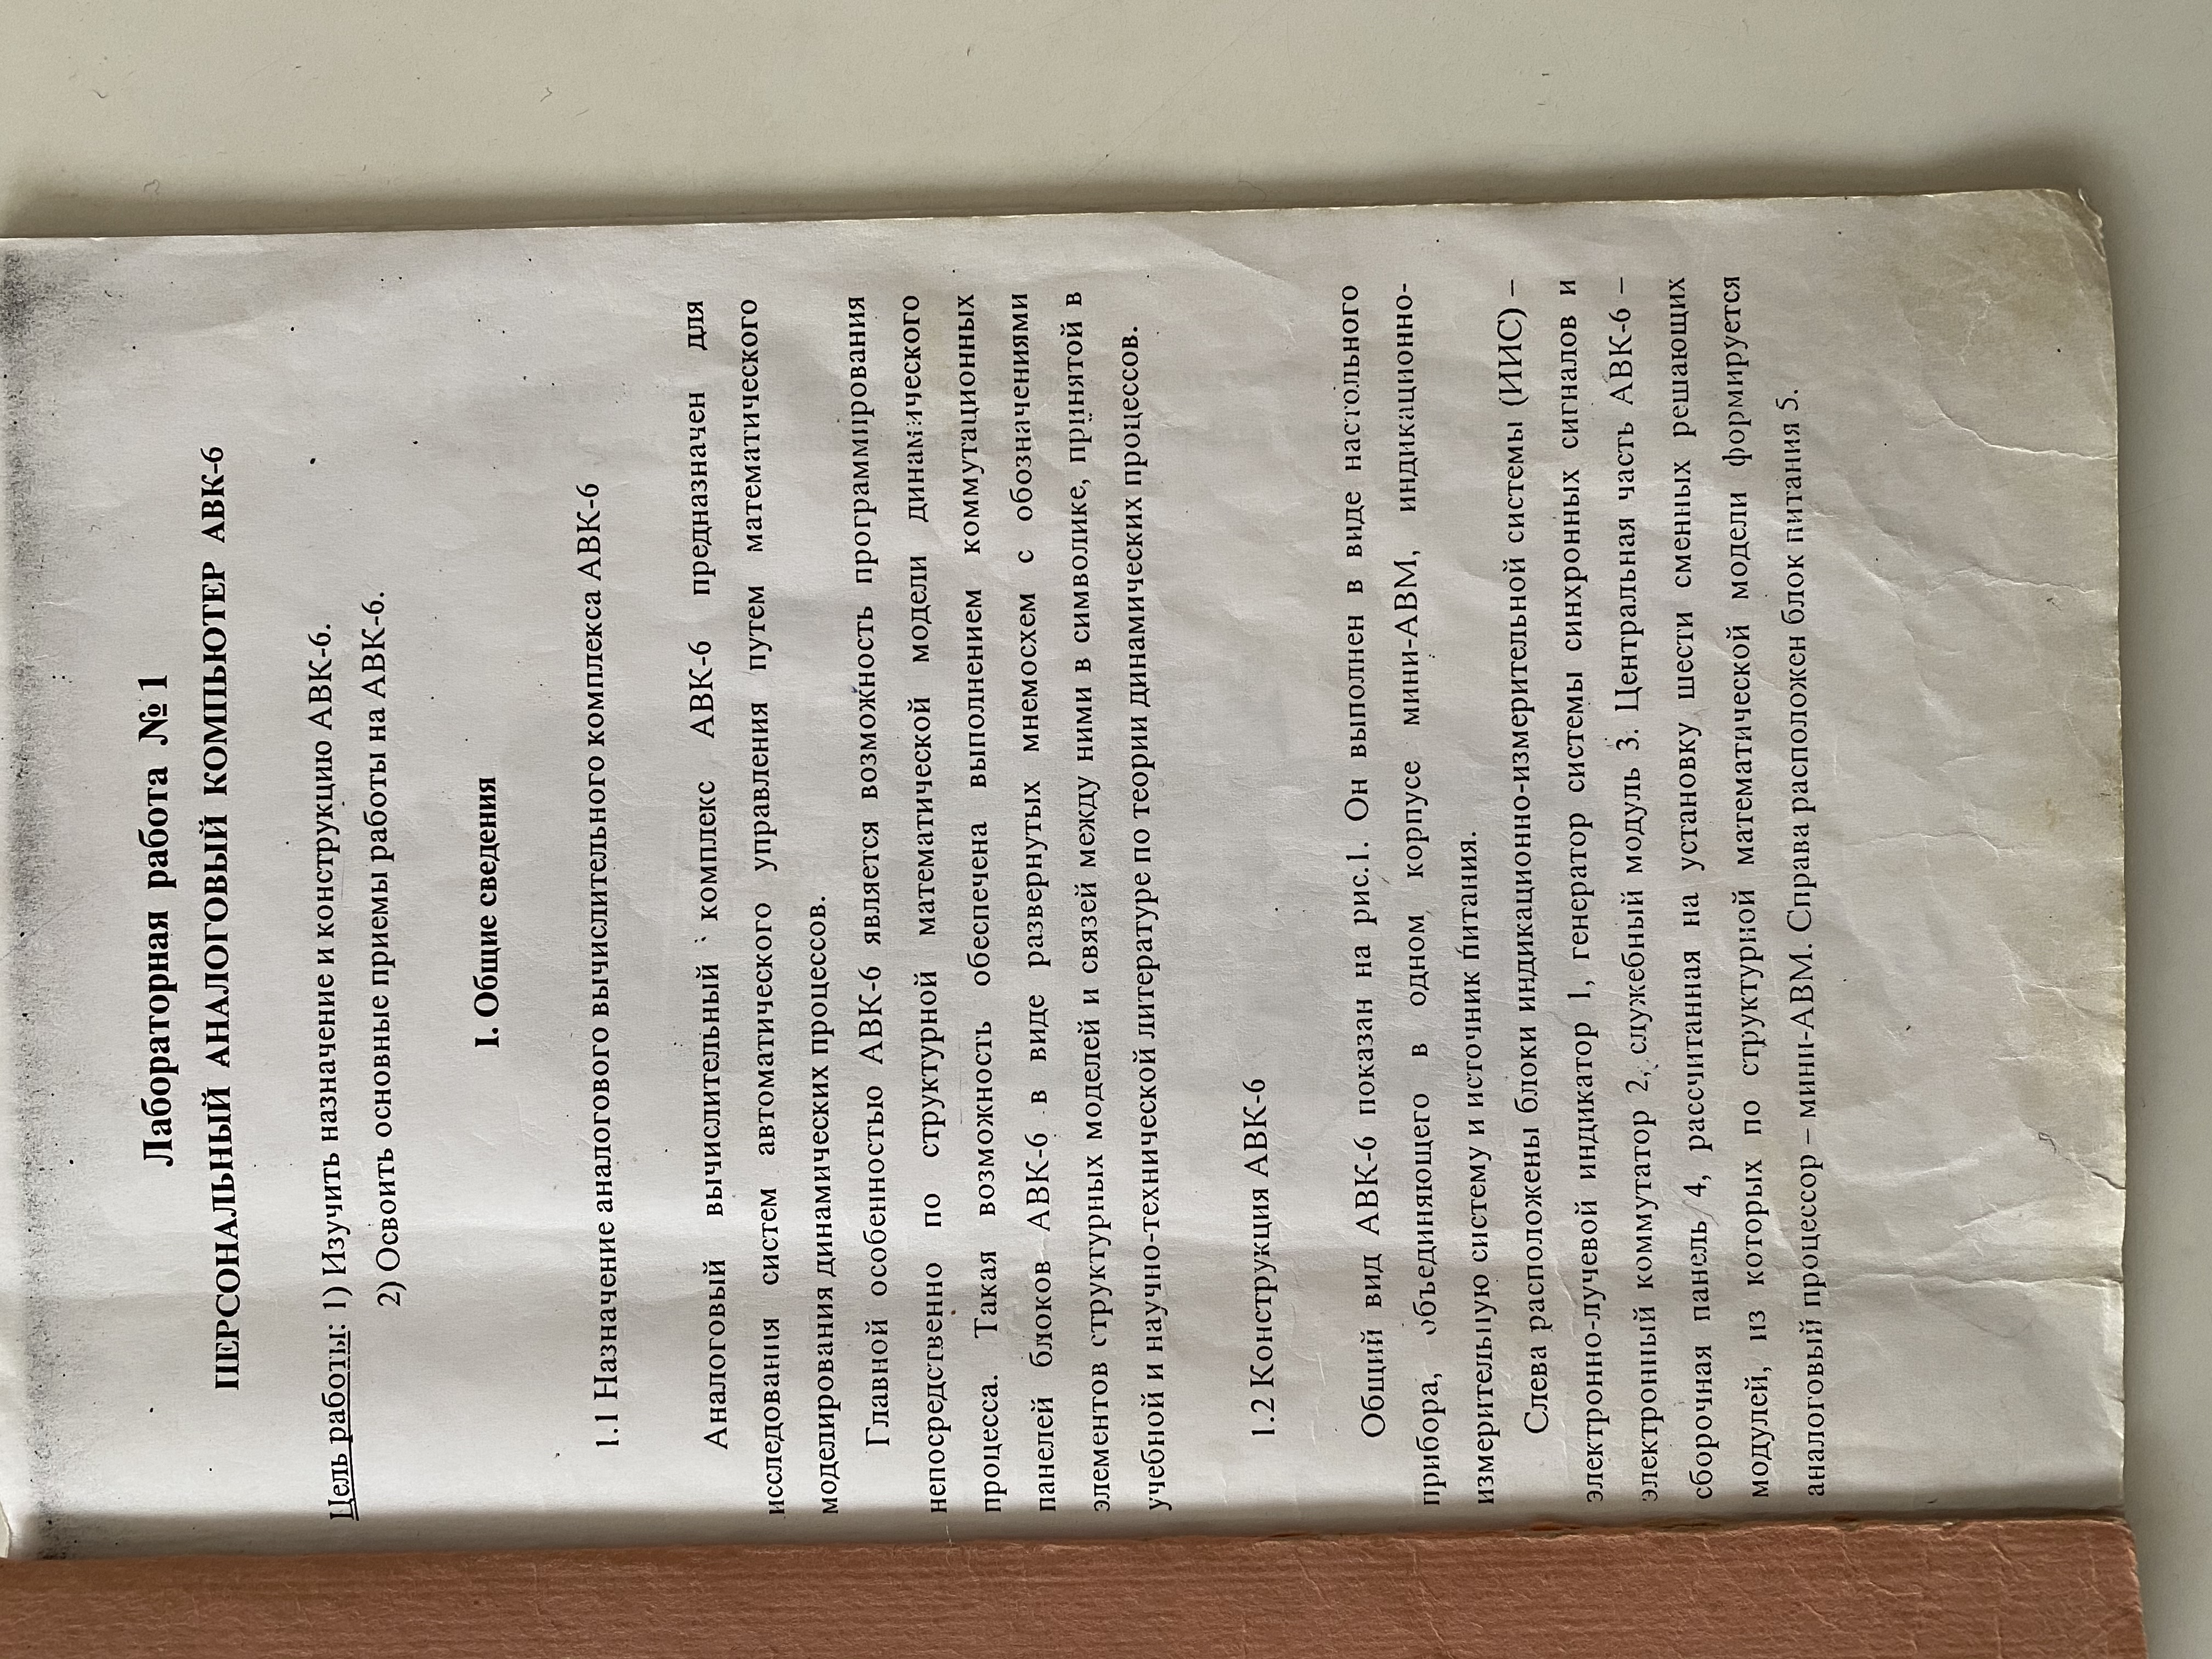
\includegraphics[width = \columnwidth]{./assets/p01.png}
        \caption{Результат виконання розробленої програми}
        \label{fig:app-res}
      \end{figure}

      Як~видно, програма коректно обчислює значення заданого виразу з~вхідними значеннями, заданими у~програмі.

  \section{Висновок}
		Виконуючи дану лабораторну роботу, ми~розробили програму для~заданої паралельної комп'ютерної системи зі~спільною пам'яттю, ознайомились із~процесом розробки паралельних алгоритмів, а~також із~моніторами у~мові програмування «\textenglish{Python}».

  \newpage
  \appendix
  \section{Програма для~розв'язку поставленої задачі}

    \inputpython{../01-solution/solution.py}{Початковий код~програмного модуля для~розв'язання задачі}{lst:source-code}

\end{document}
